% Data flow diagram
% Author: David Fokkema
\documentclass{article}
\usepackage{tikz}
\usetikzlibrary{shapes,arrows}
\usepackage{pdflscape}
\usepackage[papersize={8cm, 11cm}, text={8cm, 11cm}]{geometry}
\usetikzlibrary{decorations.text}
\usepackage{xcolor}
% \selectcolormodel{gray}

\begin{document}
\thispagestyle{empty}
%\begin{landscape}
\begin{center}
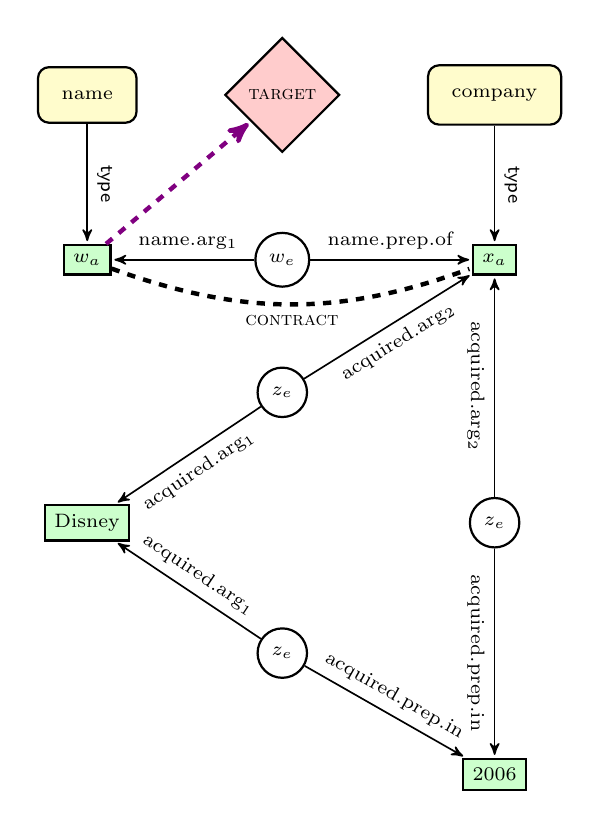
\begin{tikzpicture}[
  font=\sffamily,
  every matrix/.style={ampersand replacement=\&,column sep=1.1cm,row
sep=1cm,font=\scriptsize},
  entity/.style={draw,thick,rectangle,fill=green!20},
  word/.style={draw,thick,ellipse,fill=blue!20,},
  mediator/.style={draw,thick,circle},
  entityType/.style={draw,thick,rounded corners,fill=yellow!20,inner
sep=.3cm,font=\sffamily\scriptsize},
  mathType/.style={draw,thick,diamond,fill=red!20},
  mediatorToEntity/.style={->,>=stealth',shorten
>=1pt,semithick,black,sloped,above,font=\sffamily\scriptsize},
  typeToEntity/.style={->,>=stealth',shorten
>=1pt,semithick,black,sloped,above,font=\sffamily\scriptsize},
  wordToEntity/.style={-,>=stealth',shorten >=1pt,ultra
thick,dotted,blue,sloped,above,font=\sffamily\scriptsize},
  entityToMath/.style={->,>=stealth',shorten >=1pt,ultra
thick,dashed,violet,sloped,above,font=\sffamily\scriptsize},
  collapseEdge/.style={-,>=stealth',shorten >=1pt,ultra
thick,dashed,sloped,above,font=\sffamily\scshape,bend right=20},
  every node/.style={align=center}]

  % Position the nodes using a matrix layout
  \matrix{
    
    \node[entityType] (tName) {$\mathrm{name}$}; \& \node[mathType] (mName) {\textsc{target}}; \& \node[entityType] (tCompany) {$\mathrm{company}$}; \\
    \node[entity] (eName) {$w_a$}; \& \node[mediator] (m4) {$w_e$}; \& \node[entity] (eCompany) {$x_a$}; \\
      \& \node[mediator] (m1) {$z_e$}; \& \\
    \node[entity] (eDisney) {$\mathrm{Disney}$}; \& \& \node[mediator] (m2) {$z_e$};
\\
     \& \node[mediator] (m3) {$z_e$}; \&  \\
     \& \& \node[entity][font=\sc\scriptsize]
(e2006) {$\mathrm{2006}$}; \\
  };
 
  % words to entities
  % \draw [wordToEntity] (wDisney) edge node {}  (eDisney);
  % \draw [wordToEntity] (wCompany) edge node {}  (eCompany);
  % \draw [wordToEntity] (w2006) edge node {}  (e2006);
  
  % event word to mediators
  
  % mediator to entities
  \draw [mediatorToEntity] (m1) edge node[below] {$\mathrm{acquired.arg_1}$}  (eDisney);
  \draw [mediatorToEntity] (m1) edge node[below] {$\mathrm{acquired.arg_2}$} (eCompany);

  \draw [mediatorToEntity] (m2) edge node[below] {$\mathrm{acquired.prep.in}$}  (e2006);
  \draw [mediatorToEntity] (m2) edge node[below,rotate=180] {$\mathrm{acquired.arg_2}$} 
(eCompany);
  
  \draw [mediatorToEntity] (m3) edge node {$\mathrm{acquired.arg_1}$} 
(eDisney);
  \draw [mediatorToEntity] (m3) edge node {$\mathrm{acquired.prep.in}$}  (e2006);
  
  \draw [mediatorToEntity] (m4) edge node {\hspace{0.5em}$\mathrm{name.arg_1}$}  (eName);
  \draw [mediatorToEntity] (m4) edge node {$\mathrm{name.prep.of}$}  (eCompany);
  
  \draw [typeToEntity] (tName) edge node {type}  (eName);
  \draw [typeToEntity] (tCompany) edge node {type}  (eCompany);
  \draw [entityToMath] (eName) edge node {}  (mName);
  
  \draw [collapseEdge] (eName) edge node[below] {\scriptsize contract}  (eCompany);
\end{tikzpicture}
\end{center}

\end{document}